\documentclass[11pt,a4paper]{article}

% ------------------------------------------------------------------ fonts
\usepackage[T1]{fontenc}
\usepackage[utf8]{inputenc}
\usepackage[sc]{mathpazo}          % Palatino text + math
\linespread{1.06}
\setlength{\emergencystretch}{1.5em}
\usepackage{courier}
\usepackage{microtype}
\usepackage{textcomp}

% ------------------------------------------------------------------ layout
\usepackage[a4paper,margin=2.7cm,headheight=14pt]{geometry}
\usepackage{fancyhdr}
\usepackage{titlesec}
\usepackage{setspace}
\usepackage{enumitem}
\setlist{topsep=3pt,itemsep=2pt,parsep=0pt}

% ------------------------------------------------------------------ math & tables
\usepackage{amsmath,amssymb,amsthm}
\usepackage{booktabs}
\usepackage{array}
\usepackage{tabularx}
\usepackage{multirow}
\usepackage{longtable}
\usepackage{caption}
\captionsetup{font=small,labelfont=bf,skip=6pt}

% ------------------------------------------------------------------ figures
\usepackage{tikz}
\usepackage{pgfplots}
\pgfplotsset{compat=1.17}

% ------------------------------------------------------------------ code / algorithms
\usepackage{xcolor}
\usepackage{listings}
\usepackage{float}

\definecolor{kwcolor}{RGB}{0,60,110}
\definecolor{cmtcolor}{RGB}{110,110,110}
\definecolor{rulecolor}{RGB}{60,60,60}

\lstdefinestyle{pseudo}{
  basicstyle=\footnotesize\ttfamily,
  keywordstyle=\bfseries\color{kwcolor},
  commentstyle=\itshape\color{cmtcolor},
  morekeywords={function,procedure,return,if,then,else,for,each,while,do,end,
                require,reject,assert,input,output,let,and,or,not,in,continue,break},
  comment=[l]{//},
  mathescape=true,
  columns=fullflexible,
  keepspaces=true,
  showstringspaces=false,
  aboveskip=4pt,
  belowskip=4pt,
  xleftmargin=1.2em
}

\floatstyle{ruled}
\newfloat{algorithm}{tbp}{loa}
\floatname{algorithm}{Algorithm}

% inline wire-constant style
\newcommand{\code}[1]{\texttt{\small #1}}

% ------------------------------------------------------------------ hyperref
\usepackage[colorlinks=true,linkcolor=kwcolor,citecolor=kwcolor,urlcolor=kwcolor]{hyperref}
\hypersetup{pdftitle={Discrete: A Post-Quantum Proof-of-Work Cryptocurrency},
            pdfauthor={The Discrete developers},
            pdfsubject={Post-quantum cryptocurrency protocol}}

% ------------------------------------------------------------------ headers
\pagestyle{fancy}
\fancyhf{}
\fancyhead[L]{\small\itshape Discrete: A Post-Quantum Proof-of-Work Cryptocurrency}
\fancyhead[R]{\small\thepage}
\renewcommand{\headrulewidth}{0.3pt}

% ------------------------------------------------------------------ notation macros
\newcommand{\SHA}{\mathrm{SHA3\text{-}256}}
\newcommand{\HKDF}{\mathrm{HKDF}}
\newcommand{\KEM}{\mathrm{ML\text{-}KEM\text{-}768}}
\newcommand{\DSA}{\mathrm{ML\text{-}DSA\text{-}65}}
\newcommand{\Enc}{\mathrm{AEAD.Enc}}
\newcommand{\Dec}{\mathrm{AEAD.Dec}}
\newcommand{\concat}{\,\|\,}

\begin{document}

% ================================================================== title
\begin{titlepage}
\centering
\vspace*{1.0cm}
{\Huge\bfseries Discrete\par}
\vspace{0.3cm}
{\LARGE A Post-Quantum Proof-of-Work Cryptocurrency\par}
\vspace{0.6cm}
{\large The Discrete developers\par}
\vspace{0.15cm}
{\large \href{https://discrete.cash}{discrete.cash}\par}
\vspace{0.7cm}
{\normalsize Pre-launch protocol paper, revision 1.3 --- July 2026\par}
{\normalsize\itshape Candidate consensus constants; independent review pending\par}
\vspace{0.7cm}

\begin{minipage}{0.86\textwidth}
\small
\begin{center}\textbf{Abstract}\end{center}
\noindent
Discrete is a pre-launch proof-of-work cryptocurrency whose transaction
validation is post-quantum from genesis. Ownership uses ML-KEM-768 for private
output delivery and ML-DSA-65 for spend authorization, with deterministic seed
recovery, one-time output credentials, and nullifier-based double-spend
prevention. Amounts and the spent-output graph are transparent in Phase~1.
Mining uses DiscretePower: every candidate is signed by the coinbase
identity's ML-DSA key, and that raw signature tape is injected throughout a
modified yespower (\code{yespower-discrete}) memory-hard core, with the signature
verified before any memory-hard work runs.
The block ID commits to that randomized signature through a 32-byte SHAKE-256
witness, so distinct proofs over one unsigned candidate cannot share an ID.
This binds work and reward identity and makes conventional delegation carry the
whole per-candidate tape rather than a short digest, but it is not claimed to be a
formally strong non-outsourceable puzzle. Each
node also rejects reorganizations deeper than ten blocks relative to its local
accepted history; this weak-subjective rule protects already-connected nodes
from late private rewrites at the cost of partition wedges and operator-guided
recovery. Issuance follows a decaying exponential curve into a perpetual
approximately 2\%-per-year tail. This paper specifies the candidate protocol,
wire formats, monetary policy, recovery procedure, residual risks, and the
limits that remain before public launch and independent review.
\end{minipage}

\vfill
{\small\itshape Genesis anchor: ``Reuters 08/Jul/2026 --- Crypto firms prepare
defenses as quantum threat to encryption draws nearer''\par}
\vspace{0.6cm}
\end{titlepage}

\setcounter{tocdepth}{2}
\tableofcontents
\newpage

% ==================================================================
\section{Introduction}\label{sec:intro}

\subsection{The quantum threat to existing cryptocurrencies}

Bitcoin authorizes spending with ECDSA over secp256k1; most chains built since
use Ed25519 or close relatives. The security of every one of these schemes
reduces to the hardness of the elliptic-curve discrete-logarithm problem,
which is secure against all known classical algorithms and \emph{completely
broken} by a sufficiently large quantum computer running Shor's
algorithm~\cite{shor}: given a public key, the algorithm recovers the private
key in polynomial time. On a cryptocurrency this directly threatens spend
authorization and any classically signed control plane:

\begin{itemize}
\item \textbf{Ownership is forgeable.} Any address whose public key has been
      exposed --- every address that has ever spent, and on many chains every
      address outright --- can be drained by an adversary who forges its
      signatures.
\item \textbf{Classically signed control planes are forgeable.} A chain that
      gives checkpoint, bridge, treasury, or governance authority to an
      elliptic-curve key exposes that authority as well. This is distinct from
      proof-of-work subsidy validation, which does not ordinarily depend on an
      ownership signature.
\item \textbf{The exposure persists.} An adversary can archive exposed public
      keys today and forge ownership signatures if suitable hardware later
      matures. This is a future-forgery risk, not decryption of encrypted chain
      data.
\end{itemize}

The industry's dominant response is to plan \emph{migrations}: bolting
post-quantum signature schemes onto chains that were born classical.
Migrations of live monetary systems are slow and contentious, require flag
days, and inevitably leave a long tail of un-migrated outputs --- coins whose
owners are inactive, deceased, or unaware --- that remain permanently
vulnerable and whose eventual theft or freezing is a governance crisis waiting
to happen.

\subsection{Post-quantum from genesis}

Discrete takes the other path. It is post-quantum \textbf{from genesis}:
there is no elliptic-curve operation anywhere in its transaction validation
path, no vulnerable legacy state, no migration plan because there is nothing
to migrate. Every key, signature, and output from block~0 onward is built on
the algorithms the U.S.\ National Institute of Standards and Technology
standardized for exactly this threat: ML-KEM-768 (FIPS~203~\cite{fips203}) and
ML-DSA-65 (FIPS~204~\cite{fips204}), both at NIST Security Category~3.

The substantive technical achievement is not merely a post-quantum transparent
transaction format. It is the reconstruction of CryptoNote-style stealth
ownership~\cite{cryptonote} --- static reusable addresses, per-output one-time
credentials, deterministic recovery of an entire wallet from one seed, and
nullifier-based double-spend prevention --- using \emph{only} standardized
NIST post-quantum primitives and symmetric cryptography
(Section~\ref{sec:tx}).

\subsection{Beyond cryptography: the consensus layer}

Post-quantum keys defend against tomorrow's adversary; a young proof-of-work
chain must first survive today's. The attacks that have actually defeated
small proof-of-work coins are not cryptanalytic --- they are
\emph{hashrate-assembly} attacks: renting hashrate, incentivizing miners to
point at a hostile pool, and using the assembled majority to rewrite
confirmed history. In 2025 this reached even the largest ASIC-resistant chain
in existence, whose history was deeply reorganized by an external pool that
simply out-bid the honest network for rented and incentivized
hashrate~\cite{qubic}.

Discrete's consensus design (Section~\ref{sec:consensus}) starts from the
principle that \emph{51\% resistance cannot come from inside proof-of-work}:
any rule verifiable purely from hashrate is satisfied by whoever holds the
most of it. Discrete therefore deploys two mechanisms:

\begin{enumerate}
\item \textbf{Identity-bound signed proof-of-work} (SPoW,
      Section~\ref{sec:spow}): every unit of valid work is an ML-DSA
      signature-then-hash bound to the key that controls the block reward.
      Every nonce needs the reward identity's signature. This blocks unsigned
      reward redirection and adds a signing bottleneck to delegation, but a
      custodial operator can still sign and distribute candidate jobs. The
      mechanism descends from Karbo; operational history is not a formal
      non-outsourceability proof.
\item \textbf{Node-local first-seen depth limit}
      (Section~\ref{sec:finality}): each node records which chain it
      witnessed growing and refuses any reorganization deeper than a fixed
      finality depth, however much work the competing chain carries.
      Observation order is a resource an attacker cannot obtain by having more
      hashrate.
\end{enumerate}

\subsection{Organization and status}

Section~\ref{sec:principles} states the design principles.
Section~\ref{sec:crypto} fixes the cryptographic suite and notation.
Sections~\ref{sec:keys} and~\ref{sec:tx} specify accounts, addresses, and the
transaction family with pseudocode matching the reference implementation.
Section~\ref{sec:consensus} specifies consensus: the signed proof-of-work,
difficulty adjustment, and the finality rule with its recovery procedure.
Section~\ref{sec:monetary} specifies monetary policy and the genesis Treasury
Reserve. Section~\ref{sec:security} analyzes security and states the design's
costs. Section~\ref{sec:roadmap} describes the staged path to confidential
amounts. Appendices~\ref{app:params}--\ref{app:wire} collect the candidate
network parameters, domain-separation tags, and wire formats.

This document is a pre-launch technical overview drafted against candidate
consensus constants. The implementation, specification files, and pinned
known-answer vectors must be reconciled byte-for-byte before a launch tag; the
public release must identify the exact repository commit reviewed.

% ==================================================================
\section{Design principles}\label{sec:principles}

Discrete is deliberately \emph{compact and auditable}. The reference
implementation is a pre-launch, post-quantum, transparent-amount chain, with confidential-amount
  discretion staged as a separately reviewed and independently audited fork
(Section~\ref{sec:roadmap}). Four principles govern every choice in this
paper:

\begin{description}
\item[Standardized primitives only in consensus.] Discrete uses
  NIST-standardized post-quantum algorithms (FIPS~203, FIPS~204) and
  well-established symmetric primitives (SHA-3~\cite{fips202},
  HKDF~\cite{rfc5869}, ChaCha20-Poly1305~\cite{rfc8439}). No novel,
  un-cryptanalyzed construction sits on the critical path.
\item[Inherited mechanisms, re-evaluated.] Parts of the mining design descend
  from Karbo, but operational history is evidence rather than a proof. Discrete
  states separately what identity-bound work, local finality, and recovery do
  and do not guarantee.
\item[Objective rules separated from local state.] Emission and ownership are
  functions of public consensus data. The depth-10 reorganization limit is
  relative to a node's locally accepted history, and exceptional recovery uses
  an operator-confirmed out-of-band majority signal.
\item[Honest about what is and is not protected.] The monetary policy has no
  hard cap (by design, Section~\ref{sec:monetary}); mining is CPU-oriented
  and therefore not botnet-proof (Section~\ref{sec:spow}); finality trades a
  recoverable liveness event for protection of already-observed deep history
  (Section~\ref{sec:finality}); and Phase-1 spends are publicly linkable
  (Section~\ref{sec:ownership}). Each cost is deliberate and documented.
\end{description}

% ==================================================================
\section{Cryptographic foundations}\label{sec:crypto}

\subsection{Primitive suite}

Discrete's consensus uses exactly the primitives in
Table~\ref{tab:primitives}. Both lattice schemes are NIST Security
Category~3, a strength target comparable to AES-192, against both classical
and quantum adversaries.

\begin{table}[htbp]
\centering
\caption{Normative cryptographic suite.}
\label{tab:primitives}
\footnotesize
\begin{tabularx}{\textwidth}{@{}lllX@{}}
\toprule
\textbf{Role} & \textbf{Primitive} & \textbf{Standard} & \textbf{Sizes} \\
\midrule
View / scan key & ML-KEM-768 & FIPS 203 & pk 1{,}184\,B; sk 2{,}400\,B; ct 1{,}088\,B; ss 32\,B \\
Spend authority & ML-DSA-65 & FIPS 204 & pk 1{,}952\,B; sk 4{,}032\,B; sig 3{,}309\,B; seed 32\,B \\
Hash & SHA3-256 & FIPS 202 & output 32\,B \\
KDF & HKDF-SHA3-256 & RFC 5869 + FIPS 202 & salt $0^{32}$; $L$ as specified \\
AEAD & ChaCha20-Poly1305 & RFC 8439 (IETF) & key 32\,B; nonce 12\,B; tag 16\,B \\
Proof-of-work & DiscretePower & FIPS 202/204 + yespower-discrete & 16\,MiB scratchpad (frozen) \\
Address encoding & extended Bech32m-derived & custom length profile & HRP \code{disc} / \code{tdisc} \\
\bottomrule
\end{tabularx}
\end{table}

\noindent Two conventions apply throughout:

\begin{itemize}
\item \textbf{HKDF instantiation.} Every HKDF call is HKDF-SHA3-256 with a
  fixed salt of 32 zero bytes; the \emph{info} string is the domain tag shown
  in each derivation, and the output length is $L{=}32$ unless stated
  otherwise. Implementations must not vary salt or length.
\item \textbf{AEAD nonce.} The ChaCha20-Poly1305 nonce is 12 zero bytes.
  This is safe because every AEAD key is unique per output --- it is derived
  from a per-output KEM shared secret --- and key uniqueness makes nonce reuse
  structurally impossible rather than merely improbable.
\end{itemize}

\subsection{Notation}

$H(\cdot)$ denotes SHA3-256. $a \concat b$ denotes byte-string concatenation.
$\mathrm{LE32}(x)$ and $\mathrm{LE64}(x)$ denote 32- and 64-bit little-endian
encodings. Domain tags are ASCII strings hashed \emph{without} a trailing NUL.
$\HKDF(\mathrm{ikm}, \mathrm{info}, L)$ abbreviates
$\mathrm{HKDF\text{-}SHA3\text{-}256}(\mathrm{IKM}{=}\mathrm{ikm},
\mathrm{salt}{=}0^{32}, \mathrm{info}, L)$.
For the KEM, $(\mathit{ct}, \mathit{ss}) \leftarrow \KEM.\mathrm{Encaps}(pk)$
and $\mathit{ss} \leftarrow \KEM.\mathrm{Decaps}(sk, \mathit{ct})$; for the
signature scheme, $(pk, sk) \leftarrow \DSA.\mathrm{KeyGen}(\xi)$ with 32-byte
seed $\xi$, $\sigma \leftarrow \DSA.\mathrm{Sign}(sk, m)$, and
$\DSA.\mathrm{Verify}(pk, m, \sigma) \in \{0,1\}$.

\subsection{Domain separation}\label{sec:domains}

All key material and every consensus-critical hash in Discrete is derived
under a distinct, versioned ASCII domain tag with the prefix
\code{discrete-}, so that (i) material derived for one purpose can never be
reused for another, and (ii) material derived for Discrete can never collide
with another system --- including its own design ancestor, whose tags used the
prefix \code{karbo-pq-}. The full normative table appears in
Appendix~\ref{app:domains}; tags reserved for future phases
(\code{discrete-pq-ct-mask-v1}, \code{discrete-pq-serial-v1}) must not be used
by Phase-1 code, and unit tests pin every tag byte-for-byte. A mismatch in any
derivation between independent implementations is a chain split; known-answer
test vectors for every derivation are published with the source.

\subsection{The cost of post-quantum sizes}

Lattice keys and signatures are one to two orders of magnitude larger than
the elliptic-curve material they replace, and Discrete accepts this cost
explicitly rather than compressing it away with non-standard tricks. The
candidate consensus sizes are pinned in code and tests: a spend reveals a
1{,}952-byte ML-DSA-65
public key and a 3{,}309-byte signature; an output carries a 1{,}088-byte
ML-KEM-768 ciphertext. These sizes drive several engineering choices
documented later: coinbase outputs omit the KEM ciphertext entirely and are
recovered deterministically (Section~\ref{sec:coinbase}), saving 1{,}144
bytes per block; fees are flat rather than size-proportional
(Section~\ref{sec:fees}); and human-facing identity uses short on-chain
account numbers rather than raw addresses (Section~\ref{sec:accounts}).
% ==================================================================
\section{Keys, accounts, and addresses}\label{sec:keys}

\subsection{Deterministic key derivation from one seed}\label{sec:seed}

A Discrete account is a pair of independent post-quantum keys derived from a
single 32-byte CSPRNG master seed. Reference wallets render those bytes as a
25-word Electrum-style mnemonic. The two
branches are domain-separated so that neither key can be inferred from the
other or from the seed of the other branch:

\begin{align}
\mathit{view\_seed} &= \HKDF\bigl(\mathit{seed}_{\mathrm{master}},\;
    \text{\code{discrete-pq-view-root-v1}},\; L{=}64\bigr) \\
(\mathit{vpk}, \mathit{vsk}) &= \KEM.\mathrm{KeyGen}(\mathit{view\_seed}) \\[4pt]
\mathit{spend\_seed} &= \HKDF\bigl(\mathit{seed}_{\mathrm{master}},\;
    \text{\code{discrete-pq-spend-root-v1}},\; L{=}32\bigr) \\
(\mathit{spk}, \mathit{ssk}) &= \DSA.\mathrm{KeyGen}(\xi = \mathit{spend\_seed})
\end{align}

The view branch uses $L{=}64$ because FIPS~203 key generation consumes 64
bytes ($d \concat z$); the spend branch uses $L{=}32$ because FIPS~204 takes a
32-byte seed $\xi$. The \textbf{view key} $(\mathit{vpk}, \mathit{vsk})$
receives and audits: it decapsulates the per-output delivery ciphertexts and
can therefore see everything the account receives, but cannot spend. The
\textbf{spend key} $(\mathit{spk}, \mathit{ssk})$ is the sole spending
authority. Backing up the one master seed reconstructs the primary post-quantum
identity and every derived deposit key; recovery is a deterministic chain rescan
(Section~\ref{sec:scanning}) with no per-output secret key material stored.
The number of deposit addresses previously issued is wallet metadata rather than
seed material, so a seed-only restore must also supply that address count.

\subsection{Address format}

A Discrete address carries both public keys, so that any sender can deliver
an output (via $\mathit{vpk}$) and bind it to the recipient's spending
authority (via $\mathit{spk}$):

\begin{center}
\small
\begin{tabular}{@{}llr@{}}
\toprule
\textbf{Field} & \textbf{Content} & \textbf{Size} \\
\midrule
\code{version}       & $= 1$                                & 1\,B \\
\code{networkPrefix} & varint legacy numeric prefix (\code{0x3445db}) & 4\,B \\
\code{viewPub}       & ML-KEM-768 public key                 & 1{,}184\,B \\
\code{spendPub}      & ML-DSA-65 public key                  & 1{,}952\,B \\
\code{checksum}      & $H(\text{\code{version}} \concat \text{\code{prefix}}
                        \concat \mathit{vpk} \concat \mathit{spk})[0{:}4]$ & 4\,B \\
\bottomrule
\end{tabular}
\end{center}

The serialized address uses the \textbf{Bech32m alphabet and polymod
constant}~\cite{bip350}, plus an inner four-byte SHA3 checksum. It is not a
standard BIP-350 Bitcoin address: BIP-173's generic Bech32 profile caps strings
at 90 characters~\cite{bip173}, while a Discrete base address is approximately
5{,}043 characters. Addresses
are self-identifying by network: the mainnet human-readable prefix is
\code{disc} (addresses render as \code{disc1\ldots}) and testnet is
\code{tdisc} (\code{tdisc1\ldots}), so the two can never be confused; a
wallet rejects an address from the other network even though the underlying
keys would parse. Because the payload is over 3~KB, a rendered address runs to
several thousand characters --- intended for files, payment URIs, or
copy--paste, not transcription. It exceeds the capacity of a single standard
QR symbol; multi-frame transport would require a separate framing protocol.
Human-facing identity is
handled by the account-number layer below.

\subsection{On-chain account numbers}\label{sec:accounts}

Discrete adds an optional on-chain \textbf{account-number registry} that maps
short, human-checkable identifiers to full addresses. A user registers once by
publishing a transaction whose \code{tx\_extra} carries a registration tag
binding the identity's two public keys:
\[
\text{registration tag} \;=\; \mathrm{tag} \concat \mathit{vpk}\,(1{,}184\,\mathrm{B}) \concat \mathit{spk}\,(1{,}952\,\mathrm{B}).
\]
Consensus enforces \emph{first-registration-wins}: the first confirmed
transaction registering a given key pair is canonical, and any later attempt
is invalid. The account number is not chosen by the user; it is derived from
the registration's position in the chain --- the pair
$(\mathit{blockHeight}, \mathit{txIndex})$ --- globally unique on a given
history and resolvable by any node with no extra trust. The pair $(H,I)$ names a
\emph{position in one chain history}; to keep that position from silently
changing meaning under a reorganization, the rendered number also carries a short
\emph{fingerprint} $A$ of the registered keys. It renders in
\textbf{H-I-A-C} form,
\[
\underbrace{\mathit{height}}_{H} \text{-} \underbrace{\mathit{txIndex}}_{I}
\text{-} \underbrace{A}_{\mathrm{fingerprint}}
\text{-} \underbrace{c}_{\mathrm{check}},
\]
where $A = \mathrm{SHA3\text{-}256}(\text{\code{DISCRETE-ACCT-FP-v1}} \concat
\mathit{net} \concat \mathit{spk} \concat \mathit{vpk})_{[0{:}20\,\mathrm{bits}]}$
rendered as four Crockford Base32 characters, and $c$ is a Crockford Luhn mod-32
check character over the symbols of $H$, $I$ and $A$, so any single transcription
typo --- including one in $A$ --- is caught locally before a lookup. A resolving
conforming wallet recomputes $A$ from the keys the node returns and \emph{refuses the number
on a mismatch}, so a reorganization, or a dishonest node, that repoints $(H,I)$
to different keys cannot silently redirect a payment. Registration persists in
the node database under two
indices (key\,$\to$\,position for duplicate rejection;
position\,$\to$\,key for resolution) and rolls back across reorgs exactly
like the nullifier set (Section~\ref{sec:spending}).

\paragraph{Resolution stability under reorganization.}
The position $(H,I)$ is not a hash of the registration, so a reorganization that
replaces block $H$ can change what sits there: the adopted branch may hold the
same registration again, hold \emph{no} registration (the number stops
resolving), or hold a \emph{different} identity's keys. Two mechanisms keep this
from misdirecting a payment. First, \emph{resolution is finality-gated}: a node
returns a registration's keys only once it is more than $\Phi=10$ blocks behind
the tip (Section~\ref{sec:finality}), so a still-reorg-eligible $(H,I)$ is simply
not payable by others. Second, the fingerprint $A$ \emph{detects} any substitution
that does slip through near a partition, or on an eclipsed or newly syncing node:
the resolved keys will not reproduce $A$, and the paying wallet refuses the number
rather than sending to the replacement keys. The registry rollback itself is
intended consensus behavior, not a checksum or database fault.

The resolution RPC is intentionally positional: its request carries $(H,I)$ and
its response carries the keys plus the canonical account number reconstructed
from those keys. Consequently, \code{found=true} alone is not authorization to
pay. A remote client must require the returned canonical number, parse it, and
compare its $A$ with the user-supplied $A$; an in-process client performs the
equivalent hash comparison directly. Missing or mismatching binding data is a
hard failure. This distinction separates three states that must not be conflated:
syntactically valid, present and final on one node, and key-bound safe to pay.

First-seen finality is local and history-relative, not a global certificate, and
$A$ is only $20$ bits --- decisive against accidental or reorg-induced mismatch
(a random collision is about $2^{-20}$) but a mere speed bump against an adversary
who grinds a key pair to a chosen fingerprint. For high-value or long-lived use,
therefore, still wait $20$--$60$ confirmations, resolve through independently
operated nodes, and verify the resolved full address through a trusted channel; a
sudden ``fingerprint mismatch'' or resolution change is a stop condition, not an
automatic address update. Owners who need a durable public alias should publish a
full PQ address alongside the account number.

\paragraph{Free registration for new users.}
A new user holds no coins and cannot pay a fee, but needs an on-chain
registration to be practically payable. Discrete resolves this bootstrap
problem with a dedicated zero-fee transaction type, \code{TX\_FREE\_REG},
whose anti-spam cost is a memory-hard proof-of-work instead of a fee. A
free-registration transaction is valid iff it has no inputs and no outputs,
carries exactly one registration tag and one PoW tag, and satisfies
\begin{equation}
\begin{aligned}
\mathrm{yespower}\bigl(&\text{\code{discrete-pq-free-reg-pow-v1}}
 \concat \mathit{vpk} \concat \mathit{spk} \\
 &\concat \mathit{refBlockHash} \concat
 \mathrm{LE64}(\mathit{nonce})\bigr)_{[0:8]}
 \;\le\; \mathtt{FREE\_REG\_POW\_TARGET}.
\end{aligned}
\end{equation}
where the first eight output bytes are interpreted as a big-endian integer, both
public keys are bound so one proof cannot be replayed with different spend
identities, and $\mathit{refBlockHash}$ must be a main-chain block within the last
\code{FREE\_REG\_REF\_WINDOW} $= 60$ blocks (preventing precomputation
hoarding) and the target $\mathtt{0x00007FFFFFFFFFFF}$ implies an expected
$2^{17} = 131{,}072$ yespower evaluations --- with the 8-MiB free-registration
yespower parameters, minutes of one-time CPU work for a legitimate user, but real
CPU-hours for bulk squatting. Blocks admit at most
\code{FREE\_REG\_PER\_BLOCK} $= 100$ such transactions, and the mempool caps
pending registrations at $2{,}000$ so zero-fee traffic can never crowd out
paid transactions.

\subsection{Unlimited deposit addresses from one key}\label{sec:deposits}

Exchanges and merchants need a distinct address per customer or invoice.
Classical chains answer with subaddress schemes that multiply scan work or
key state; Discrete instead binds a 32-bit \textbf{routing index} $T$ into
each output's delivery. $T$ is not a key: spend authority is unchanged. Because
$T$ also enters the AEAD key derivation, the wallet enumerates its issued $T$
window after one ML-KEM decapsulation; each candidate costs one context hash and
one AEAD attempt. A deposit identifier renders as
\textbf{H-I-A-T-C} (the base account plus fingerprint plus index plus a Crockford
Luhn check character over all of $H$, $I$, $A$ and $T$), which can never alias the
three-dash base form. One account
can therefore hand every counterparty its own deposit address without a new
registration, while persisting the issued-address count needed to bound scans
and seed-only recovery.

For deployments that prefer distinct spend keys per deposit, the wallet layer
additionally supports an \emph{aggregated-multikey} family: per-deposit
ML-DSA-65 spend keys
\begin{equation}
\begin{split}
\xi_i &= \HKDF\bigl(\mathit{seed}_{\mathrm{master}},\;
\text{\code{discrete-pq-deposit-spend-v1}} \concat \mathrm{LE32}(i),\; 32\bigr),\\
(\mathit{spk}_i, \mathit{ssk}_i) &= \DSA.\mathrm{KeyGen}(\xi_i),
\end{split}
\end{equation}
all sharing the single view key, so scanning still costs one decapsulation
per output. Both derivations are cemented: changing the domain, the index
encoding, or the HKDF parameters would strand existing deposits on recovery.

% ==================================================================
\section{Transactions}\label{sec:tx}

Discrete has one transaction version and four transaction types:
\code{TX\_COINBASE} (0x00, block reward), \code{TX\_PQ} (0x01, ordinary
transfer), a permanently reserved type 0x02, and \code{TX\_FREE\_REG} (0x03,
Section~\ref{sec:accounts}). This section specifies the life of a
\code{TX\_PQ} output: construction, delivery, scanning, spending, and
validation.

\subsection{Output construction}\label{sec:output}

\paragraph{Per-output randomness.}
Every output carries a secret 32-byte blinding value $\rho$, drawn fresh from
a CSPRNG by the sender. $\rho$ is delivered encrypted to the recipient and
revealed only when the output is spent; it binds the output's credentials to
that specific output so no other output's material can be substituted.

\paragraph{Consensus-enforced output uniqueness.}
A stable per-output identifier, \emph{outContext}, is computed before any key
derivation. Uniqueness must be \emph{enforced}, not assumed: a malicious
sender who could replay the same KEM ciphertext and output index in two
transactions would produce two outputs with identical credentials, of which
only one could ever be spent. Discrete folds the transaction's
\emph{inputs hash} into the context; since consensus guarantees a given set
of UTXOs is spent at most once, the inputs hash is a uniqueness source that
costs no new fields:
\begin{align}
\mathit{inputsHash} &= H\Bigl(\text{\code{discrete-pq-inputs-hash-v1}}
  \concat \bigl(\mathit{prevTxid}_j \concat \mathrm{LE32}(\mathit{prevOutIndex}_j)\bigr)_{j=1..n}\Bigr) \\
\mathit{outContext} &= H\Bigl(\text{\code{discrete-pq-out-context-v1}}
  \concat \mathit{inputsHash} \concat \mathit{kemCt}
  \concat \mathrm{LE32}(i) \concat \mathrm{LE64}(T)\Bigr)
\label{eq:outcontext}
\end{align}
where $i$ is the output's index in the transaction and $T$ is the routing
index of Section~\ref{sec:deposits} ($T{=}0$ for ordinary payments).

\paragraph{Delivery, binding, and authenticated encryption.}
The sender encapsulates to the recipient's view key, derives a one-time AEAD
key, and seals $\rho$ and $T$; the public amount is bound into the
authentication tag as associated data, so any in-flight tampering with the
amount, the context, or the routing hint makes the output invisible to the
recipient rather than wrongly credited:
\begin{align}
(\mathit{kemCt}, \mathit{ss}) &\leftarrow \KEM.\mathrm{Encaps}(\mathit{vpk}) \\
k_{\mathrm{aead}} &= \HKDF\bigl(\mathit{ss},\;
  \text{\code{discrete-pq-aead-key-v1}} \concat \mathit{outContext},\; 32\bigr) \\
\mathit{encPayload} &= \Enc\bigl(k_{\mathrm{aead}},\; \mathrm{nonce}{=}0^{12},\;
  \mathrm{aad}{=}\mathit{outContext} \concat \mathrm{LE64}(a),\;
  \rho \concat \mathrm{LE64}(T)\bigr)
\end{align}
yielding 40 bytes of ciphertext plus a 16-byte tag (56 bytes on the wire,
consensus-enforced). Finally the output commits to the recipient's spending
authority:
\begin{equation}
\mathit{spendCommit} = H\bigl(\text{\code{discrete-pq-spend-commit-v1}}
 \concat \mathit{spk} \concat \rho\bigr).
\label{eq:spendcommit}
\end{equation}
The on-chain output is
$\bigl(\mathrm{LE64}(a),\, \mathrm{LE64}(\mathit{unlockHeight}),\,
\mathrm{0x10},\, \mathit{kemCt},\, \mathit{encPayload},\,
\mathit{spendCommit}\bigr)$ --- 1{,}193 bytes. Note what is
\emph{absent}: neither public key appears. Until the output is spent, an
observer sees only a hash commitment and an encapsulation that is
indistinguishable from random without $\mathit{vsk}$ --- this is Discrete's
post-quantum stealth receiving.

\begin{algorithm}[tbp]
\caption{\textsc{CreateOutput} --- sender side (per output $i$ of amount $a$ to address $(\mathit{vpk}, \mathit{spk})$, routing index $T$).}
\label{alg:createoutput}
\begin{lstlisting}[style=pseudo]
function CreateOutput(inputsHash, i, a, unlockHeight, vpk, spk, T):
    rho $\leftarrow$ CSPRNG(32)
    (kemCt, ss) $\leftarrow$ ML-KEM-768.Encaps(vpk)
    ctx  $\leftarrow$ SHA3-256("discrete-pq-out-context-v1" $\|$ inputsHash $\|$ kemCt
                     $\|$ LE32(i) $\|$ LE64(T))
    k    $\leftarrow$ HKDF(ss, "discrete-pq-aead-key-v1" $\|$ ctx, 32)
    enc  $\leftarrow$ AEAD.Enc(k, nonce=$0^{12}$, aad=ctx $\|$ LE64(a), msg=rho $\|$ LE64(T))
    sc   $\leftarrow$ SHA3-256("discrete-pq-spend-commit-v1" $\|$ spk $\|$ rho)
    // sender self-check: run the receiver predicate (Alg. 2) on (kemCt, enc, sc)
    // using ss directly; abort on any mismatch
    return Output{ a, unlockHeight, 0x10, kemCt, encPayload=enc, spendCommit=sc }
\end{lstlisting}
\end{algorithm}

\paragraph{Garbage outputs.}
A malicious sender can emit an output whose fields are well-formed but
meaningless. This is inherent to every stealth-address system: the node
cannot detect it without the recipient's view secret. The recipient's wallet
handles it correctly and silently --- decapsulation of a garbage ciphertext
returns a pseudorandom secret, the derived AEAD key is wrong, tag
authentication fails, and the output is discarded before it ever appears in a
balance. The only party harmed is the sender, whose coins are burned; the
fee requirement makes this an expensive way to spam.

\subsection{The ownership model, and why it has a long-term spend key}
\label{sec:ownership}

Discrete's design ancestor (the Karbowanec PQ proposal, ``KDSK'') derived a
\emph{per-output} spend key directly from the KEM shared secret:
\[
\xi_i = \HKDF(\mathit{ss}, \cdot), \qquad
(\mathit{pk}_i, \mathit{sk}_i) = \DSA.\mathrm{KeyGen}(\xi_i).
\]
This is elegant --- no spend key in the address,
per-output keys for free --- and \textbf{unsound}: a KEM establishes the
\emph{same} shared secret for both parties, and the \emph{sender} runs
Encaps and therefore knows $\mathit{ss}$. Since $\mathit{sk}_i$ is a
deterministic function of $\mathit{ss}$ and public data, the sender can
re-derive the spend secret of the output it just created and race the
recipient to spend it. Every payment would be clawable; no payment would
ever be final. The flaw is structural: the sender must be able to compute the
spend \emph{public} key to build the commitment, so any spend key derived
from sender-known material is sender-spendable. A recipient-only secret must
enter the spend path --- and the only place it can live is the address.

Discrete therefore gives each identity a \textbf{long-term ML-DSA-65 spend
keypair} (Section~\ref{sec:seed}), publishes $\mathit{spk}$ in the address,
and binds outputs to it via the commitment of
Eq.~\eqref{eq:spendcommit}. The sender knows $\mathit{spk}$ (it is public)
and chooses $\rho$, so it can still construct the output --- but it cannot
sign, because it lacks $\mathit{ssk}$. The resulting properties:

\begin{itemize}
\item \textbf{Receiving stays private.} An output carries only
  $\mathit{spendCommit}$; $\rho$ is encrypted and $\mathit{spk}$ is not on
  chain until a spend. Unspent outputs are unlinkable to any address, and even
  after one spend reveals $\mathit{spk}$, the identity's \emph{other} unspent
  outputs stay unlinkable (linking them would require their secret $\rho$
  values).
\item \textbf{Spends are publicly linkable.} Spending reveals
  $\mathit{spk}$, so spends under the same spend authority are linkable, and the
  spent output is identified exactly. Aggregated-multikey wallets compartmentalize
  deposits under distinct derived spend keys, but every revealed input still makes
  the spent-output graph transparent. This is the deliberate, documented Phase-1
  trade-off (Section~\ref{sec:roadmap}).
\item \textbf{Quantum-safe finality of payment.} Only the holder of
  $\mathit{ssk}$ --- never the sender --- can authorize a spend.
\end{itemize}

\subsection{Scanning and wallet recovery}\label{sec:scanning}

Scanning mirrors the CryptoNote mental model --- try every output, and let
cryptography sort ownership --- with the AEAD tag and the spend commitment as
the two gates. Recovery from seed is the same procedure run from genesis.

For single-key-index wallets, the candidates share one spend public key and
enumerate issued $T$ values. Aggregated-multikey addresses always use $T=0$;
the implementation decrypts once and tests the resulting commitment against
the primary and known derived deposit spend keys. In both modes ML-KEM
decapsulation is performed only once per output.

\begin{algorithm}[tbp]
\caption{\textsc{Scan} --- recipient side, per transaction $\mathit{tx}$ with wallet scan candidates $(T,\mathit{spk})$.}
\label{alg:scan}
\begin{lstlisting}[style=pseudo]
function ScanTx(tx, vsk, candidates):
    ih $\leftarrow$ inputsHash(tx.inputs)      // from the tx being scanned
    for each (i, out) in tx.outputs where out.type == 0x10:
        ss  $\leftarrow$ ML-KEM-768.Decaps(vsk, out.kemCt)      // garbage ct $\Rightarrow$ random ss
        for each (T, spk) in candidates:
            ctx $\leftarrow$ SHA3-256("discrete-pq-out-context-v1" $\|$ ih
                            $\|$ out.kemCt $\|$ LE32(i) $\|$ LE64(T))
            k   $\leftarrow$ HKDF(ss, "discrete-pq-aead-key-v1" $\|$ ctx, 32)
            m   $\leftarrow$ AEAD.Dec(k, $0^{12}$, aad=ctx $\|$ LE64(out.amount), out.encPayload)
            if m = $\perp$: continue          // not ours, or tampered: hard discard
            (rho, T$'$) $\leftarrow$ parse m;  require T$'$ == T
            if SHA3-256("discrete-pq-spend-commit-v1" $\|$ spk $\|$ rho)
                    $\neq$ out.spendCommit:
                continue       // ownership gate: never credit without this
            record { txid, i, out.amount, out.unlockHeight, rho, ctx, T }
\end{lstlisting}
\end{algorithm}

Two invariants are wallet-critical. First, an output is never credited as
spendable until the spend-commitment check passes --- AEAD success alone
proves delivery, not ownership. Second, no spend secret is stored per output:
the wallet record is $\{$txid, index, amount, $\rho$, context, $T\}$, and the
long-term $\mathit{ssk}$ is re-derived from the seed on demand.

\subsection{Spending, the signing digest, and nullifiers}\label{sec:spending}

\paragraph{Signing digest.}
To spend, the owner constructs the full unsigned transaction and signs a
digest that binds the \emph{entire} prefix --- version, type, unlock height,
every input's outpoint and revealed credentials, every output byte, the
\code{tx\_extra} blob, and the fee:
\begin{equation}
\begin{split}
d = H\bigl(&\text{\code{discrete-pq-tx-sign-v1}} \concat \mathit{ver}
 \concat \mathit{txType} \concat \mathrm{LE64}(\mathit{unlockHeight})
 \concat \mathrm{LE32}(n_{\mathrm{in}}) \\
&\concat \bigl(\mathit{prevTxid}_j \concat \mathrm{LE32}(\mathit{prevOutIndex}_j)
 \concat \mathit{spk}_j \concat \rho_j\bigr)_{j}
 \concat \mathrm{LE32}(n_{\mathrm{out}}) \\
&\concat \bigl(\mathrm{type}_i \concat \mathrm{LE64}(a_i)
 \concat \mathrm{LE64}(u_i) \concat \mathit{kemCt}_i
 \concat \mathit{encPayload}_i \concat \mathit{spendCommit}_i\bigr)_{i} \\
&\concat \mathrm{LE32}(|\mathit{extra}|) \concat \mathit{extra}
 \concat \mathrm{LE64}(\mathit{fee})\bigr)
\end{split}
\label{eq:digest}
\end{equation}
Each input then carries $\sigma_j = \DSA.\mathrm{Sign}(\mathit{ssk}_j, d)$.
Binding every prefix field that enters the txid closes malleability: a
relayer who mutates the type, a lock, the extra field, or any output
invalidates every signature.

\paragraph{Nullifiers.}
Double-spend prevention uses a \emph{nullifier} --- a unique, unforgeable
marker for the spent output, Discrete's post-quantum analogue of a key image:
\begin{equation}
\mathit{nf} = H\bigl(\text{\code{discrete-pq-nullifier-v1}} \concat
\mathit{spk} \concat \rho \concat \mathit{prevTxid} \concat
\mathrm{LE32}(\mathit{prevOutIndex})\bigr).
\label{eq:nullifier}
\end{equation}
Nullifiers are \textbf{computed by every validating node from revealed
fields and never serialized in the transaction} --- a node never trusts a
provided value, which removes a class of malleability and
inconsistent-validation attacks outright. Binding the spent outpoint makes
the nullifier unique per output even when two outputs share
$(\mathit{spk}, \rho)$; this matters because coinbase outputs use a
\emph{publicly recomputable} $\rho$ (Section~\ref{sec:coinbase}) that could
otherwise be replayed into a colliding output to brick the original. The
outpoint is already revealed in the spending input, so nothing extra leaks.
The nullifier set is persisted keyed by block height, so a reorg rolls it
back exactly (delete at orphaned heights, re-apply along the adopted chain).

\begin{algorithm}[tbp]
\caption{\textsc{Spend} --- wallet side, spending stored records $R_1..R_n$ to outputs $O_1..O_m$.}
\label{alg:spend}
\begin{lstlisting}[style=pseudo]
function Spend(records, outputs, fee, extra):
    (spk, ssk) $\leftarrow$ deriveSpendKeys(seed$_{master}$)   // re-derived; never persisted
    for each R in records:
        inputs += { R.prevTxid, R.prevOutIndex, authPub=spk, rhoReveal=R.rho }
    d $\leftarrow$ txSigningDigest(ver=1, TX_PQ, unlockHeight, inputs, outputs,
                          extra, fee)          // Eq. (13)
    for each input j:  $\sigma_j$ $\leftarrow$ ML-DSA-65.Sign(ssk, d)
    discard ssk from memory
    return SignedTx{ prefix, $\sigma_1..\sigma_n$ }
\end{lstlisting}
\end{algorithm}

\subsection{Consensus validation rules}\label{sec:validation}

\begin{algorithm}[tbp]
\caption{\textsc{ValidateTxPQ} --- node side, for each \code{TX\_PQ} transaction.}
\label{alg:validate}
\begin{lstlisting}[style=pseudo,basicstyle=\scriptsize\ttfamily]
function ValidateTxPQ(tx, chainState):
    require 1 $\le$ |inputs| $\le$ 32, 1 $\le$ |outputs| $\le$ 64, size(tx) $\le$ 256 KiB
    require |tx.extra| $\le$ 4096  and  tx.fee $\ge$ feeFloor(|tx.extra|)   // Sec. 5.8
    d $\leftarrow$ txSigningDigest(tx)              // Eq. (13)
    total_in $\leftarrow$ 0
    for each input j in tx.inputs:
        out $\leftarrow$ chainState.lookup(j.prevTxid, j.prevOutIndex)
        require out exists, type $\in$ {0x10, 0x11}, mature, height $\ge$ out.unlockHeight
        require SHA3-256("discrete-pq-spend-commit-v1" $\|$ j.authPub $\|$ j.rhoReveal)
                == out.spendCommit
        nf $\leftarrow$ SHA3-256("discrete-pq-nullifier-v1" $\|$ j.authPub $\|$ j.rhoReveal
                        $\|$ j.prevTxid $\|$ LE32(j.prevOutIndex))
        require nf $\notin$ chainState.nullifierSet    // double-spend check
        require ML-DSA-65.Verify(j.authPub, d, $\sigma_j$) == 1
        total_in += out.amount
    for each output i:  require wellFormed(i) and canonicalDenomination(i.amount)
    require total_in == $\sum_i$ tx.outputs[i].amount + tx.fee   // exact balance
    for each input j:  chainState.nullifierSet.insert(nf$_j$, height)
\end{lstlisting}
\end{algorithm}

Validation (Algorithm~\ref{alg:validate}) is exact: the balance equation
admits no tolerance, signatures are verified against the revealed
$\mathit{authPub}$ that the spend commitment binds, and the fee floor and
size caps are consensus rules, not relay policy.

\subsection{Canonical denominations}\label{sec:denoms}

Every output amount must be one of 64 \textbf{canonical denominations}:
$d \cdot 10^{e}$ atoms for digit $d \in \{1..9\}$ and decade
$e \in \{0..6\}$ (63 values), plus a cap of $10^{7}$ atoms
($=100{,}000$~XDS). Wallets decompose any payment greedily from the largest
denomination down; because the smallest denomination is the atomic unit
(1 atom $= 0.01$~XDS), every amount is exactly representable and no dust case
exists. Uniform denominations serve two purposes: the on-chain amount universe
is identical across wallet implementations (no wallet fingerprinting by split
pattern), and the set is \emph{forward-compatible} --- the planned
confidential-amount design (Section~\ref{sec:roadmap}) proves membership of a
hidden amount in exactly this 64-element table, so outputs created today
already live in the right universe and need no migration.

\subsection{Per-output time-locks}\label{sec:timelocks}

Each output carries its own \code{unlockHeight} (0 = none): the output cannot
be spent until the chain reaches that height. Because the lock is per-output
--- distinct from the legacy per-transaction lock --- a single transaction can
release some funds immediately and vest others over time. The field is bound
into the signing digest~\eqref{eq:digest} and the txid, so it is not
malleable; it deliberately does \emph{not} enter \eqref{eq:outcontext} or the
AEAD associated data, keeping ownership and delivery independent of the lock.
The genesis Treasury Reserve (Section~\ref{sec:treasury}) uses exactly this
mechanism, and it is available to any user for vesting and escrow-style
payments.

\subsection{Fees}\label{sec:fees}

PQ transactions are intrinsically large --- a spend costs 5{,}329 bytes per
input and 1{,}193 bytes per output (Table~\ref{tab:sizes}). Output count is not
a clean proxy for discretionary bloat because the wallet decomposes ordinary
amounts into canonical denominations: for example, 1{,}234 atoms naturally
becomes four outputs of 1{,}000, 200, 30, and 4 atoms. Charging per output would
therefore tax the decimal structure of the payment. Discrete retains a
predictable \textbf{flat base fee}, with a surcharge on the free-form
\code{tx\_extra} field:
\begin{equation}
\mathrm{feeFloor}(x) \;=\; f_{\min} \;+\;
\begin{cases}
0, & x \le 3200 \\[2pt]
f_{\min} \cdot \bigl\lceil (x - 3200)/100 \bigr\rceil, & x > 3200
\end{cases}
\label{eq:fee}
\end{equation}
with $f_{\min} = 1$ atom $= 0.01$~XDS and
$x = |\code{tx\_extra}|$ (capped at
4{,}096 bytes). The 3{,}200-byte free allowance is sized so that every
protocol-required extra --- in particular a paid account-number registration
tag of 3{,}137 bytes --- fits without surcharge. A maximum-sized extra produces
a 0.10-XDS consensus floor; the separate wallet UI sanity cap is 1.00~XDS, so
an explicitly chosen fee may be higher than the floor. Input/output counts and total transaction size remain
hard-capped; miners choose which transactions to include; and the dynamic
block-size penalty reduces subsidy above the median. A maximal transaction can
still pay the same base fee as a small transfer. That is an explicit policy
trade-off, not a claim that all size is unavoidable; changing it requires
separate economic analysis rather than assuming per-byte pricing is correct.

\subsection{Payment proofs}\label{sec:proofs}

A wallet creates a version-2 payment proof for each external recipient when it
sends a PQ transaction. The Bech32m artifact names the network and transaction,
hashes the recipient's spend authority, and reveals the output indices and
$\rho_i$ values needed to recompute Eq.~\eqref{eq:spendcommit} and total the
public amounts. It proves that those on-chain outputs were committed to the
claimed spend key; it does not prove ML-KEM delivery, attribution to a particular
subaddress index, receipt, or later control of the funds. Proofs and recipient
labels are ordinary sent-payment metadata in the encrypted wallet cache. They
are written on the next normal wallet save, cannot be reconstructed from a
mnemonic or a chain rescan, and may be lost if the process crashes first, so a
proof needed as durable evidence should be exported after sending.

\subsection{Transaction sizes}

\begin{table}[htbp]
\centering
\caption{Wire sizes (consensus-enforced).}
\label{tab:sizes}
\footnotesize
\begin{tabular}{@{}lrl@{}}
\toprule
\textbf{Element} & \textbf{Bytes} & \textbf{Composition} \\
\midrule
Input (\code{PqInput}) & 5{,}329 & outpoint $32{+}4$ $\concat$ $\mathit{spk}$ 1952 $\concat$ $\rho$ 32 $\concat$ sig 3309 \\
Output (\code{PqOutput}, 0x10) & 1{,}193 & amt 8 $\concat$ lock 8 $\concat$ tag 1 $\concat$ $\mathit{kemCt}$ 1088 $\concat$ payload 56 $\concat$ commit 32 \\
Coinbase output (0x11) & 49 & amount 8 $\concat$ lock 8 $\concat$ tag 1 $\concat$ commit 32 \\
Typical 1-in/2-out transfer & $\approx$ 7{,}735 & $+\,{\approx}20$ B envelope \\
Caps per \code{TX\_PQ} & --- & $\le 32$ inputs, $\le 64$ outputs, $\le 256$ KiB \\
\bottomrule
\end{tabular}
\end{table}

A coinbase output omits the KEM ciphertext and encrypted payload entirely ---
1{,}144 bytes saved per block --- because its recipient is recovered
deterministically from public data (Section~\ref{sec:coinbase}).
% ==================================================================
\section{Consensus}\label{sec:consensus}

A proof-of-work chain is secured by hashrate, and hashrate is mercenary: it
flows to whatever pays most, and it can be rented, incentivized, or brought to
bear against a small chain for the few hours needed to rewrite its history.
Discrete's consensus starts from a principle drawn from that history:

\begin{quote}\itshape
51\% resistance cannot come from inside proof-of-work. A unique algorithm, a
decentralized pool, or any rule verifiable purely from hashrate can always be
satisfied by whoever holds the most hashrate --- because hashrate is the only
Sybil-resistant resource proof-of-work exposes, and the attacker has a
majority of it.
\end{quote}

Discrete narrows two attack paths: identity-bound work adds friction to generic
delegation, while a local depth limit makes already-connected nodes refuse a
late deep rewrite. Neither mechanism removes the underlying majority assumption,
and their guarantees are stated separately below.

\subsection{Identity-bound signed proof-of-work}\label{sec:spow}

Rental markets and pools depend on delegable work. Discrete makes delegation
less direct by requiring the reward identity to participate in every attempt,
but does not claim that this alone eliminates custodial pools.

Discrete's proof-of-work is \textbf{DiscretePower}, a composition of
SHAKE-256, ML-DSA-65, and \code{yespower-discrete} --- yespower 1.0 with the raw
signature tape injected at the specified S-box generation, large-memory fill,
and read/write lookup sites of its memory-hard loops.
Let $h(B)$ be the block-hashing blob of block $B$ (major/minor version,
timestamp, $\mathit{prevHash}$, nonce, and the transaction Merkle root; it
excludes the signature), and let $d_H,d_M,d_P,d_F$ be the four pinned domain
strings in Appendix~\ref{app:domains}. The exact construction is
\begin{align}
H_B &= \mathrm{SHAKE256}(d_H \concat h(B), 64) \\
m_B &= \mathrm{SHAKE256}(d_M \concat H_B, 64) \\
\sigma_B &= \DSA.\mathrm{Sign}(\mathit{ssk}_{\mathrm{miner}}, m_B) \\
\mathit{tape}_B &= \sigma_B \concat \mathtt{0x80} \concat \mathtt{0x00} \concat \mathtt{0x00} \\
P &= \mathrm{SHAKE256}(d_P, 32) \\
Y_B &= \mathrm{yespowerDiscrete}_{N=4096,\,r=32}(H_B;\mathrm{pers}=P;\mathrm{tape}=\mathit{tape}_B) \\
\mathrm{PoW}(B) &= \mathrm{SHAKE256}(d_F \concat H_B \concat Y_B, 32)
\label{eq:pow}
\end{align}
and the block is valid if $\mathrm{PoW}(B) \cdot D \le 2^{256}$ for current
difficulty $D$, if $\sigma_B$ verifies against the miner spend public key
carried in the coinbase \code{extra} \emph{before} any \code{yespower-discrete} work runs,
and if the coinbase pays that same key (Section~\ref{sec:coinbase}). Because the
signature covers the nonce, \emph{every} candidate requires a fresh ML-DSA
signature, and the whole $3{,}312$-byte tape is consumed across the frozen
injection schedule, beginning before the first S-box entry is stored and
continuing through the state-dependent memory phases. No memory-hard prefix is
reusable across signatures. The signature is the reward binding; there is no
separate reward signature. With an all-zero tape the injection is a no-op and
\code{yespower-discrete} collapses to stock yespower 1.0.

The block ID commits to the signature through a separable witness. Let
$C_B$ be the unsigned block-hashing blob (header plus transaction-tree
commitment, excluding $\sigma_B$). The identity is
\begin{align}
W_B &= \mathrm{SHAKE256}(d_W \concat \sigma_B,\, 32) \\
\mathrm{BlockID}(B) &= \mathrm{SHAKE256}\bigl(d_I \concat \mathrm{LE64}(|C_B|)
  \concat C_B \concat W_B,\, 32\bigr),
\end{align}
with $d_W,d_I$ the pinned witness and block-identity domains
(Appendix~\ref{app:domains}). The construction is not circular: $\sigma_B$
signs $m_B$, a function of $C_B$ only, and the ID is computed afterward. Two
distinct valid signatures over one header therefore yield \emph{distinct} block
IDs, eliminating the same-ID proof aliasing that a signature-excluding ID would
admit while preserving randomized signatures as independent mining attempts;
and because each child's $\mathit{prevHash}$ is its parent's ID, a
checkpoint pin transitively commits to every block signature beneath it, which
is what makes checkpoint-anchored fast sync (Section~\ref{sec:finality}) sound.
The block ID is an identifier only: consensus admission verifies $\sigma_B$ and
recomputes the DiscretePower PoW for every new ID. A duplicate lookup may skip
revalidation only for the exact proof-bearing ID already stored; a different
signature has a different $W_B$ and therefore cannot hit that entry except by a
SHAKE-256 collision. The implementation derives $W_B$ on demand from the full
signature and exposes it in block-detail RPC responses.

\paragraph{Signature pruning.}
Each block carries its $3{,}309$-byte ML-DSA-65 PoW signature, which at the
$90$-second target ($\approx 960$ blocks/day) accrues at roughly
$1.16$~GB/year. The separable witness makes a future pruned-storage format
possible: retaining $W_B$ is sufficient to reconstruct the block ID after
discarding $\sigma_B$. It is \emph{not} sufficient to re-verify the ML-DSA
signature or the signature-dependent PoW. The current implementation therefore
retains every full signature, does not persist $W_B$ as independent block
metadata, and requires the full $3{,}309$ bytes in the block wire format.
Shipping pruning would require an explicit database representation for $W_B$,
a distinct pruned-block serving format, and a reviewed trust/bootstrap policy;
the depth limit $\Phi$ alone is not a cryptographic proof that historical work
may be discarded. Signature pruning is consequently a design option, not a
shipped feature or present consensus guarantee.

\begin{algorithm}[tbp]
\caption{\textsc{Mine} --- one attempt loop (per thread).}
\label{alg:mine}
\begin{lstlisting}[style=pseudo]
function Mine(template B, difficulty D, spend keys (spk, ssk)):
    while mining requested:
        if node is syncing: pause
        if last peer disconnected: stop hashing, retain request, wait for sync
        B.nonce $\leftarrow$ next nonce
        H $\leftarrow$ SHAKE256(dH $\|$ hashingBlob(B), 64)
        m $\leftarrow$ SHAKE256(dM $\|$ H, 64)
        $\sigma$ $\leftarrow$ ML-DSA-65.Sign(ssk, m)       // re-sign EVERY candidate
        tape $\leftarrow$ $\sigma \|$ 0x80 $\|$ 0x00 $\|$ 0x00
        Y $\leftarrow$ yespower-discrete$_{4096,32}$(H, pers=SHAKE256(dP, 32), tape)
        pow $\leftarrow$ SHAKE256(dF $\|$ H $\|$ Y, 32)
        if pow $\cdot$ D $\le 2^{256}$:  submit(B, $\sigma$); break
\end{lstlisting}
\end{algorithm}

The construction buys three concrete properties:

\begin{itemize}
\item \textbf{Reward-identity binding and delegation friction.} A candidate is
  valid only with a signature from the reward-controlling key, so an unsigned
  worker cannot redirect the reward and a conventional pool cannot expose one
  template with a freely variable nonce range. A custodial operator can still
  sign batches of nonce candidates, distribute signed jobs, accept
  lower-difficulty shares, and pay workers off-chain. The signing service must
  scale with aggregate attempt rate; this is friction, not a proof of strong
  non-outsourceability. Formally strong constructions instead make effective
  outsourcing give the worker an undetectable way to steal the winning
  reward~\cite{nonoutsourceable}.
\item \textbf{CPU-oriented memory hardness.} \code{yespower-discrete}'s 16-MiB
  scratchpad ($N{=}4096$, $r{=}32$) is the memory-hardness mechanism,
  targeting commodity CPUs rather than claiming hardware equality. Because it
  is a new yespower-derived algorithm, independent benchmarking and review of
  its hardware ratios remain advisable; the parameters are frozen for the
  launch release. The personalization tag is fixed and Discrete-specific, so
  work produced for any other chain cannot be reused, precompute-shared, or
  merge-mine confused with Discrete's.
\item \textbf{Tip-binding for free.} $\mathit{prevHash}$ is inside the signed,
  hashed header, so valid work exists only relative to the current chain
  head; mining requires tracking the tip with no extra machinery.
\end{itemize}

Discrete states the limits plainly: CPU-oriented memory hardness does not prove
permanent ASIC resistance or exclude botnets and farms, and identity binding
does not prove that purpose-built custodial pools are impossible.

\subsection{Coinbase bound to the block signer}\label{sec:coinbase}

Consensus requires each non-genesis block's \emph{single} coinbase output to
pay the very key that signed the block. The binding uses a
\emph{canonical, publicly recomputable} blinding value:
\begin{align}
\rho_C &= H\bigl(\text{\code{discrete-coinbase-rho-v1}} \concat
        \mathit{spk}_{\mathrm{signer}} \concat \mathrm{LE32}(\mathit{height})
        \concat \mathrm{LE32}(i)\bigr) \label{eq:rhoc}\\
\text{require:}\quad & \mathit{coinbase.spendCommit} \;=\;
   H\bigl(\text{\code{discrete-pq-spend-commit-v1}} \concat
   \mathit{spk}_{\mathrm{signer}} \concat \rho_C\bigr)
\end{align}
with output index $i=0$ for normal blocks. Anyone can verify the equality
from public data, so \emph{you cannot mine to a key you do not hold}: the
identity that performs the work is the identity that is paid. This is an
identity-binding property, not one half of a proof of non-outsourceability.
Because $\rho_C$ is public (unlike a
normal output's secret $\rho$), the nullifier's outpoint
binding~\eqref{eq:nullifier} guarantees distinct nullifiers even for outputs
sharing $(\mathit{spk}, \rho)$. Wallets recover mined rewards
deterministically --- recompute $\rho_C$ for own $\mathit{spk}$ at each
height, one constant-time hash comparison per candidate, no KEM
decapsulation --- which is why coinbase outputs omit the 1{,}144 bytes of
delivery machinery. The genesis block (height 0) is the sole exception to
signature validation: it is a fixed candidate constant carrying the Treasury Reserve
(Section~\ref{sec:treasury}) to 21 independent keys, with $i = 0..20$ giving
each batch a distinct $\rho_C$.

\subsection{Difficulty adjustment}\label{sec:difficulty}

Discrete retargets every block with \textbf{LWMA-1}~\cite{lwma} over a window
of $N = 60$ blocks --- the algorithm adopted across small proof-of-work chains
precisely because it reconverges quickly after hashrate swings. With target
spacing $T = 90$\,s, solve times $t_j$ (clamped to $[0, 6T]$, out-of-sequence
timestamps monotonized) and average difficulty $\bar{D}$ over the window:
\begin{equation}
L = \sum_{j=1}^{N} j \cdot \min(t_j,\, 6T), \qquad
L \ge \tfrac{N^2 T}{20}, \qquad
D_{\mathrm{next}} \;=\; \frac{\bar{D}\, \cdot\, N(N{+}1)\,T\, \cdot\, 99}{200\,L}\,,
\end{equation}
i.e.\ a linearly weighted moving average that gives recent blocks the most
weight, with a $+5\%$ trim factor ($99/200$ rather than $1/2$) and a floor
that caps the downward step. Block version 1, the only active version, rejects a
timestamp more than $3T$ in the future and requires it to exceed the median of
the previous 11 timestamps. The separate 60-block value is the LWMA difficulty
window, not the median-time-past window.

\subsection{Block-size limits and capacity growth}\label{sec:blocksize}

Discrete separates predictable long-term capacity growth from short-term
demand signaling. At height $h$, the cumulative serialized size of the
coinbase and all ordinary transactions is bounded by the absolute consensus
cap
\begin{equation}
C(h) = 1{,}000{,}000 +
\left\lfloor\frac{h \cdot 524{,}288}{350{,}400}\right\rfloor
\quad\text{bytes},
\label{eq:blockcap}
\end{equation}
where 350{,}400 is the expected number of blocks per year at the 90-s target.
The network therefore starts at exactly 1{,}000{,}000 bytes and grows smoothly
by 512~KiB per target year: the cap is 1{,}524{,}288 bytes at year one,
2{,}048{,}576 at year two, and 6{,}242{,}880 at year ten. Integer division
applies this growth in small height-indexed steps rather than annual jumps.

Independently, let
\begin{equation}
M = \max\!\left(\operatorname{median}(s_{h-100},\ldots,s_{h-1}),
1{,}000{,}000\right)
\end{equation}
be the effective median of the preceding 100 cumulative block sizes. Blocks
at or below $M$ receive the full subsidy and fees; between $M$ and $2M$ the
CryptoNote quadratic size penalty applies to both; above $2M$ reward
construction fails. A valid block must therefore satisfy
\begin{equation}
s_h \le \min(C(h),\,2M).
\end{equation}
The reference miner targets at most $1.25M$ in fee-paying transactions and
measures the actual post-quantum coinbase before finalizing a template. If
coinbase overhead would cross $C(h)$, it removes transactions and rebuilds the
template. The absolute cap supplies auditable long-run growth, while the
median penalty imposes an economic cost until sustained recent use supports
larger blocks. Changing the constants in Eq.~\eqref{eq:blockcap} changes block
validity and requires a coordinated consensus upgrade after launch.

\subsection{Local first-seen depth limit}\label{sec:finality}

Identity-bound work does not stop an attacker who funds a majority or operates
a signing pool. Discrete additionally uses local observation order: a node can
remember the history it already accepted and refuse a late competing branch.
This protects that node's prior view; it does not create a globally objective
certificate shared across partitions, new nodes, or eclipsed nodes.

\paragraph{The rule.} Let $\mathcal{C}$ be a node's current main chain with
tip height $h$, and let $\mathcal{C}'$ be any competing chain whose fork
point is at height $f$. The node applies:
\begin{equation}
\text{adopt } \mathcal{C}' \iff
W(\mathcal{C}') > W(\mathcal{C})
\;\wedge\;
h - f \le \Phi,
\qquad \Phi = \mathtt{FINALITY\_DEPTH} = 10,
\end{equation}
with $W(\cdot)$ cumulative work. A reorganization deeper than $\Phi$ blocks
($\approx$ 15 minutes at the 90-s target) is \textbf{refused regardless of
work}. A chain withheld in private and published late --- the classic deep
reorg and the end state of selfish mining --- is rejected by every node on the
ground that it was not seen first by that node. Blocks buried $\Phi$ deep are
locally final relative to that accepted history.

\paragraph{Mandatory rule, subjective input.} The depth is a consensus
parameter enforced by every node, not a runtime option, but the current chain
to which it is applied is local state. Connected nodes that observed the same
history make the same decision; partitions or eclipses can produce conflicting
locally final histories. An exchange using $\Phi$ confirmations must still
monitor independent peers and tip freshness.

\paragraph{The stated cost, bounded.} A node that continued \emph{producing}
blocks while isolated for longer than $\Phi$ blocks --- a sustained partition,
or a miner mining while disconnected --- can wedge onto a minority fork that
its own finality rule then refuses to abandon. Discrete bounds this cost in
three layers:

\begin{enumerate}
\item \textbf{Scope.} The wedge affects only nodes that were both isolated
  \emph{and} actively extending their own fork past $\Phi$. A node that
  merely went offline holds a prefix of the true chain and syncs forward
  normally; divergence shallower than $\Phi$ self-heals by ordinary reorg,
  accelerated by LWMA retargeting.
\item \textbf{Prevention in code.} The built-in miner pauses while the node is
  syncing and stops hashing when the last peer disconnects while retaining the
  requested mining state (Algorithm~\ref{alg:mine}). It resumes automatically
  only after a peer reconnects and the node reports synchronization. An explicit
  zero-peer start remains permitted to bootstrap a fresh network, and explicit
  stop clears the retained request. This prevents the ordinary connected miner
  from extending an isolated fork, but it does not detect every partition or
  eclipse that retains stale peers.
\item \textbf{First-class recovery.} On refusing a finality-violating reorg,
  the node raises a persistent \code{finality\_fork\_warning} exposing the
  local and competing tips, the divergence height, and the \emph{peer split}
  (how many peers offer the competing chain --- a human diagnostic, never an
  input to validity). The operator confirms the majority chain out-of-band
  (block explorer, independent nodes) and runs a single guarded command,
  \code{resync\_to\_majority --confirm}, which pops the local chain to just
  below the divergence height and resyncs. The command refuses to run unless
  the warning is set, so it cannot be abused to force an ordinary deep reorg
  by hand. Recovery is deliberate and operator-confirmed, never automatic.
  The out-of-band majority check is a weak-subjectivity assumption and an
  operator trust boundary, not a pure on-chain validity rule.
\end{enumerate}

The trade is explicit: refusal protects a connected node's already-observed
history, while a partition can produce conflicting locally final views that
require social recovery. The procedure is recoverable, but consensus alone
cannot prove which partition is the majority; exchanges must pause operations
until independent observations agree.

\subsection{Why the reference implementation includes no decentralized pool}\label{sec:nopool}

Decentralized pooling (p2pool and relatives) solves \emph{payout variance},
and solves it well --- but a pool of any kind shares each block's reward across
recent contributors and therefore reintroduces delegated work. DiscretePower
makes that arrangement less direct because each candidate is signed by the
reward identity; it does not make a custodial pool impossible. Nor can a
share-chain be rescued by consensus membership rules
or by applying first-seen finality to it: a membership rule is still
verifiable only from hashrate (a majority attacker runs their own
share-chain), and first-seen finality only rejects history that arrives
\emph{late} --- an attacker who mines a hostile share-chain openly and
continuously, as the 2025 attacker did, is first-seen-valid at every height.
The empirical record is pointed: the one major chain that relied on
decentralized pooling for mining decentralization is the one that was deeply
reorganized in 2025, through exactly the aggregation door SPoW keeps shut.

Discrete therefore manages variance on the solo side: a short 90-second block
interval keeps solo payouts on a human timescale, and the reference wallet
surfaces accumulated mining progress between blocks. This is a weaker
variance tool than a shared pool, accepted knowingly --- the security it
preserves is ranked above the convenience it costs.

\subsection{Network layer}\label{sec:network}

Transactions propagate with \textbf{Dandelion++}~\cite{dandelion} stem-phase
routing (epoch 600\,s, 2 stems, stem probability 0.9, embargo timeout
173\,s), narrowing the network-layer link between a transaction and its
origin IP. Default ports are 9330 (P2P) and 9331 (RPC). An optional
DNS-checkpoint channel (\code{checkpoints.discrete.cash}) lets maintainers
publish signed checkpoints; records are verified against a compiled-in
allowlist of \emph{post-quantum} signer addresses (ML-DSA-65 over a
domain-separated digest, any-of-$N$ so signers can rotate without emergency
releases) and the mechanism fails closed --- it ships disabled until a signer
is provisioned, and checkpoints can only ever \emph{confirm} history within
the finality rule, never override it.

% ==================================================================
\section{Monetary policy}\label{sec:monetary}

\subsection{The emission function}

Discrete's issuance is a pure function of consensus state, recomputed and
enforced exactly by every node. Let $A$ be the total atoms in circulation
after the parent block (\emph{alreadyGeneratedCoins}), $S =
2{,}100{,}000{,}000$ atoms ($= 21{,}000{,}000$~XDS) the exponential-curve
target, $k = 18$ the emission speed factor, and $B = 350{,}400$ the expected
blocks per year ($960$/day at the 90-s target). The base block reward is
\begin{equation}
R(A) \;=\; \max\Bigl(\;
\underbrace{\bigl\lfloor (S - A) \cdot 2^{-k} \bigr\rfloor}_{\text{exponential phase}}
,\;
\underbrace{\Bigl\lfloor \frac{2\,\lfloor A/100\rfloor}{B} \Bigr\rfloor}_{\text{perpetual tail}}
\;\Bigr),
\label{eq:emission}
\end{equation}
(with the exponential term set to a vestigial 100 atoms once $A \ge S$;
in practice the tail overtakes it long before that point). The coinbase must
equal $R(A)$ plus collected fees, adjusted by the block-size penalty,
\emph{exactly}: a block that mints one atom too many \textbf{or too few} is
rejected. There is no discretionary and no hidden issuance.

\subsection{Two phases}

\textbf{Exponential phase.} Early on, each block mints
$2^{-18} \approx 1/262{,}144$ of the remaining distance to $S$. The genesis
reserve already places $A_0=105{,}000{,}000$ atoms
($1{,}050{,}000$~XDS) in circulation, so the first
ordinary block reward is $\lfloor(S-A_0)/2^{18}\rfloor = 7{,}610$ atoms
$=76.10$~XDS; the often-quoted 80.10~XDS is only the hypothetical value at
$A=0$. Supply follows $A(t) \approx S-(S-A_0)e^{-t/\tau}$ with time constant
$\tau = 2^{18}$ blocks $\approx 273$ days, so the reward decays smoothly ---
halving roughly every $2^{18}\ln 2 \approx 181{,}700$ blocks
($\approx$ 6.2 months) --- with no cliff-edge halvings.

\textbf{Perpetual tail.} The tail term --- Milton Friedman's $k$-percent
rule~\cite{friedman} applied at 2\% per year --- overtakes the decaying
exponential when $A \approx 0.9851\,S \approx 20.69$ million XDS, roughly
3.1 years after genesis, at a per-block reward of $\approx 1.18$~XDS. From
then on the reward is 2\% of an ever-growing base spread over the year's
blocks: supply grows without bound at a long-run rate of $\sim$2\% per annum,
and the \emph{rate} is what is fixed. $S$ is therefore explicitly \textbf{not
a supply ceiling}; it is the parameter that shapes the early curve.

\begin{figure}[tbp]
\centering
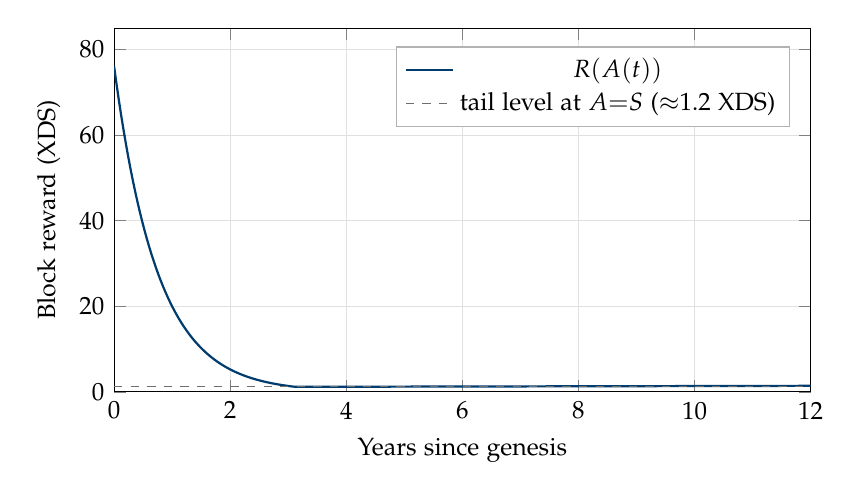
\begin{tikzpicture}
\begin{axis}[
  width=0.86\textwidth, height=6.2cm,
  xlabel={Years since genesis}, ylabel={Block reward (XDS)},
  xmin=0, xmax=12, ymin=0, ymax=85,
  grid=major, grid style={black!12},
  tick label style={font=\small}, label style={font=\small},
  legend style={font=\small, at={(0.97,0.95)}, anchor=north east, draw=black!30},
]
\addplot[color=kwcolor, thick, domain=0:12, samples=300]
  { max( 76.10 * exp(-x/0.7481), 1.18 * exp(0.02*(x-3.114)) ) };
\addlegendentry{$R(A(t))$}
\addplot[color=cmtcolor, dashed, domain=0:12, samples=2] {1.199};
\addlegendentry{tail level at $A{=}S$ ($\approx$1.2 XDS)}
\end{axis}
\end{tikzpicture}
\caption{Per-block reward over time: smooth exponential decay from 76.10~XDS
(reward half-life $\approx$ 6 months) into the perpetual $\sim$2\%/yr tail,
which crosses over at $\approx$ 20.69M~XDS supply ($\approx$ 3.1 years) and
thereafter grows slowly with the base. No halving cliffs; no terminal
subsidy collapse.}
\label{fig:emission}
\end{figure}

\subsection{Why a perpetual tail}

\begin{itemize}
\item \textbf{It funds security forever.} There is always a block subsidy,
  so miner revenue never collapses to fees alone --- avoiding the
  long-term security-budget problem hard-capped chains face as subsidies
  vanish, which for a chain whose whole premise is surviving the
  \emph{next} decades would be a self-inflicted wound.
\item \textbf{It targets stable, low, predictable inflation.} A fixed 2\% of
  supply is a shrinking real burden relative to economic activity over time,
  approximating a constant money-growth rule rather than engineered scarcity
  followed by engineered famine.
\item \textbf{It is fully auditable.} $R(A)$ is a pure function of consensus
  state; anyone can recompute the exact emission at any height.
\end{itemize}

\subsection{Units and parameters}

\begin{center}
\small
\begin{tabularx}{\textwidth}{@{}lX@{}}
\toprule
Units & 2 decimals; $1$ XDS $= 100$ atoms \\
Block target & 90 seconds \\
Exponential-curve target $S$ & 21{,}000{,}000 XDS (shapes the curve; \textbf{not a cap}) \\
Emission speed factor $k$ & 18 \\
First post-genesis block reward & 76.10 XDS \\
Long-run tail & $\sim$2\%/year, perpetual ($\approx$1.2 XDS/block at crossover) \\
\bottomrule
\end{tabularx}
\end{center}

\subsection{The Treasury Reserve: transparent and vested}\label{sec:treasury}

The genesis block allocates a \textbf{Treasury Reserve of 1{,}050{,}000 XDS
--- 5\% of the exponential-curve target} --- to fund development, audits,
infrastructure, exchange listings, documentation, and grants. Its terms are
enforced by the chain, not by promise:

\begin{itemize}
\item The reserve counts \emph{within} the emission target: it reduces the
  ongoing block reward rather than being minted on top.
  \textbf{There is no ICO, no private sale, and no separate developer tax.}
\item It is mostly locked at genesis. It vests as \textbf{21 batches of
  50{,}000 XDS}, with the first batch available immediately and one additional
  batch unlocking each quarter over five years, using the
  per-output time-lock of Section~\ref{sec:timelocks}: batch $k$ (1-based)
  unlocks at height $(k{-}1) \times 87{,}600$ ($\approx$ one quarter of
  90-s blocks), so batch 1 is spendable at genesis and batch 21 at height
  1{,}752{,}000 $\approx$ 5.0 years.
\item The 21 recipients are independent single-key post-quantum accounts held
  in cold storage; their spend public keys are committed in the candidate
  genesis constant, so no node or peer can alter the allocation. Each stripped
  \code{CoinbaseOutput} stores
  $\mathrm{spendCommit}(\mathit{spk}_i,
  \mathrm{coinbaseRho}(\mathit{spk}_i,0,i))$ with no KEM ciphertext; anyone can
  regenerate and verify the bytes.
\item The genesis coinbase \code{extra} embeds a dated headline ---
  \emph{``Reuters 08/Jul/2026 --- Crypto firms prepare defenses as quantum
  threat to encryption draws nearer''} --- Discrete's analogue of Bitcoin's
  Chancellor headline and a statement of purpose. The frozen block timestamp is
  15~July 2026 13:49:13 UTC. Neither timestamp nor headline proves the public
  announcement time or absence of private mining; the headline only establishes
  that the candidate artifact could not have been assembled before its publication.
\end{itemize}

This is a deliberate, documented departure from a zero-premine model: a young
chain needs cryptographic audits and infrastructure, and a transparent,
capped, on-chain-vested reserve funds that without hidden issuance or
discretionary control.
% ==================================================================
\section{Security analysis}\label{sec:security}

\subsection{Threat model}

Discrete defends against a network adversary who controls message timing and
a minority of nodes; a mining adversary who can rent, incentivize, or own
hashrate up to and beyond a majority; malicious transaction counterparties
(senders and recipients); and a \emph{quantum-capable archival adversary} who
records the entire chain today and later gains a cryptographically relevant
quantum computer. Against the last, Discrete's ownership rests on the
Module-LWE/Module-SIS assumptions underlying ML-KEM-768 and ML-DSA-65 at
Category~3; symmetric primitives (SHA3-256, ChaCha20-Poly1305) retain
comfortable margins against Grover-type speedups, whose quadratic advantage
is further blunted in practice by memory-hardness in the PoW path. Discrete
does not defend against: compromise of a user's seed or endpoint; a global
network adversary performing traffic correlation beyond what Dandelion++
mitigates; or hardware-scarcity attacks on CPU mining (botnets, large farms),
which are stated openly as outside the design's reach.

\subsection{Ownership and supply integrity}

\begin{itemize}
\item \textbf{Spend unforgeability} reduces to ML-DSA-65 existential
  unforgeability: authorizing a spend requires a signature over the full
  digest~\eqref{eq:digest} under the exact public key bound into the output's
  commitment~\eqref{eq:spendcommit}. Substituting a different key requires a
  SHA3-256 second preimage.
\item \textbf{Payment finality against the sender.} The sender can construct
  but never spend an output (Section~\ref{sec:ownership}) --- resolving the
  clawback flaw in the ancestor design and making receipt final on
  confirmation.
\item \textbf{Double-spend prevention} reduces to the collision resistance of
  the nullifier hash~\eqref{eq:nullifier} and exactness of the persisted
  nullifier set (height-keyed, reorg-rolled). Nullifiers are node-derived and
  never on the wire, so no malleated value can desynchronize validators.
\item \textbf{Supply exactness.} Every block's coinbase is checked to equal
  $R(A)$~+~fees exactly~\eqref{eq:emission}; a one-atom deviation in either
  direction is invalid. Emission cannot be inflated by any party, including
  miners.
\item \textbf{Output integrity in flight.} Amount, context, and routing index
  are bound into the AEAD tag; any mutation makes the output invisible to its
  recipient rather than mis-credited. Output-credential uniqueness is
  consensus-enforced through the inputs hash~\eqref{eq:outcontext}.
\end{itemize}

\subsection{Attack catalogue}

\begin{table}[tbp]
\centering
\caption{Transaction-layer attacks and dispositions.}
\label{tab:attacks}
\small
\begin{tabularx}{\textwidth}{@{}lllX@{}}
\toprule
\textbf{Attack} & \textbf{Node detects} & \textbf{Wallet detects} & \textbf{Disposition} \\
\midrule
Malformed field sizes & yes, at admission & --- & consensus rejects; all blob sizes fixed \\
Garbage output (valid sizes) & no & yes (AEAD tag) & inherent to stealth systems; sender burns own coins; recipient unaffected \\
Amount tampered in flight & no & yes (AAD) & hard discard at scan; recipient unaffected \\
KEM-ct replay across txs & yes & --- & \emph{outContext} binds inputs hash; same ct in another tx yields different credentials \\
$\rho$ reuse & not a threat & --- & fresh KEM ct $\Rightarrow$ unique context; outpoint-bound nullifier stays unique \\
Nullifier precollision & infeasible & --- & SHA3-256 preimage resistance \\
Tx malleation by relayer & yes & --- & digest~\eqref{eq:digest} binds the full prefix; signatures break on any mutation \\
Registration squatting & rate-limited & --- & first-reg-wins + memory-hard PoW + per-block and mempool caps \\
\bottomrule
\end{tabularx}
\end{table}

\subsection{Consensus attacks}

\textbf{Hashrate rental / hostile pool aggregation.} Generic unsigned jobs do
not work because every nonce needs the reward identity's signature. A custom
custodial pool can nevertheless retain that key, sign candidate jobs at
aggregate rate, and pay shares off-chain. The construction adds operational
friction and a signing bottleneck; it does not eliminate aggregation.

\textbf{Self-funded majority, withheld chain.} An attacker who owns a
majority and mines privately produces a heavier chain. A connected node that
already accepted the honest history refuses it at depth $> \Phi$. New,
offline, partitioned, or eclipsed nodes may hold a different local view, and a
majority can censor new blocks while it persists.

\textbf{Selfish mining.} Withholding beyond $\Phi$ is rejected by nodes that
already observed the competing history; within $\Phi$, ordinary cumulative-work
selection applies. Profitability is not proved here and depends on propagation,
hashrate, and local observation.

\textbf{Timestamp and difficulty games.} Solve-time clamping to $[0, 6T]$,
monotonization, the $N^2T/20$ floor on $L$, the active $3T$ future limit, and
the median of the previous 11 timestamps constrain timestamp leverage.
Adversarial simulation is still required before launch.

\textbf{Partition wedges (the accepted residual).} A network segment that
mines in isolation past $\Phi$ wedges and must run the recovery procedure of
Section~\ref{sec:finality}. After a connected node loses its last peer, the
reference miner stops and later resumes only after reconnection and sync; the
explicit zero-peer bootstrap path, an eclipsed miner with stale peers, or a
connected minority segment can still continue.
Operator-confirmed recovery chooses which local history to discard.

\subsection{Costs stated plainly}

For the reader auditing trade-offs, the complete list of what Discrete
\emph{gives up}, each deliberate: no hard supply cap (a 2\%/yr tail is the
price of a permanent security budget); publicly linkable spends and
transparent amounts in Phase 1; a protocol composition that is test-covered
but not yet independently audited; CPU-oriented mining that is not botnet- or
farm-proof; possible custodial pooling despite identity binding; and
weak-subjective finality that can wedge or conflict under partitions and needs
operator-guided recovery.

% ==================================================================
\section{Roadmap: staged discretion}\label{sec:roadmap}

Discrete is a pre-launch, post-quantum, transparent-amount reference chain.
Privacy refinements are research proposals for separately reviewed and audited
forks. Nothing in this section is consensus until it is implemented, independently
reviewed, and frozen.

\subsection{Confidential amounts}

The one planned refinement is \emph{cash-like discretion over magnitudes}: a
payer should not reveal their remaining balance to a payee who can currently
read the change output. The direction, recorded in the development
specifications:

\begin{itemize}
\item The output's plaintext amount is replaced by a committed
  \textbf{denomination bundle}: $K$ fixed slots, each a lattice commitment to
  one member of the canonical 64-denomination set of
  Section~\ref{sec:denoms} (zero-padded to uniform $K$, so structure leaks no
  digit count). Commitments are Module-SIS additive,
  \begin{equation}
  C = \mathbf{A}\,\mathbf{r} + v\,\mathbf{u} \pmod q,
  \end{equation}
  binding under Module-SIS and homomorphic in $v$, with $q$ chosen larger
  than any feasible transaction value so modular balance implies integer
  balance --- eliminating the carry-proof machinery whose retrofitted checks
  produced audit findings in comparable deployed systems.
\item Membership of each slot in the denomination table is shown with a
  lattice \textbf{one-out-of-many proof}; balance is one aggregate identity,
  \begin{equation}
  \sum_{\mathrm{inputs}} C_j \;-\; \sum_{\mathrm{outputs}} C_i \;-\;
  \mathit{fee}\cdot\mathbf{u} \;=\; \mathbf{A}\,\mathbf{r}_\Delta,
  \end{equation}
  proven to open to zero hidden value.
\item The ownership model is untouched: ML-KEM delivery, ML-DSA spend
  authority, and nullifier double-spend prevention carry over; the signing
  digest additionally binds the value-commitment root so commitments cannot
  be swapped under a valid signature, and the encrypted payload authenticates
  against it so recipients reject tampered commitments.
\end{itemize}

The audit focus is supply integrity --- denomination membership soundness,
balance, overflow bounds, commitment binding, and malleability --- and the
fork ships only after independent review. The accepted structural cost is
quantization: an amount needing more nonzero digits than $K$ slots splits
across outputs, so output count can correlate weakly with amount complexity.

\subsection{On untraceability}

Discrete deliberately does \emph{not} pursue hiding the transaction graph.
The flow of funds stays transparent and publicly auditable --- a property that
keeps the chain compatible with exchange and compliance expectations, and
consistent with its identity as post-quantum \emph{cash} rather than an
anonymity system. Confidential amounts add discretion over magnitudes only;
they do not make the chain untraceable, and that boundary is by design, not a
limitation awaiting a later fix.

% ==================================================================
\section{Related work}\label{sec:related}

\textbf{Bitcoin}~\cite{bitcoin} established proof-of-work consensus and the
UTXO model; its ECDSA ownership and its fee-only terminal security budget are
the two long-horizon liabilities Discrete addresses.
\textbf{CryptoNote}~\cite{cryptonote} introduced stealth addresses, one-time
output keys, and key images; Discrete reconstructs precisely this receiving
model on standardized lattice primitives, with nullifiers in place of key
images. \textbf{Karbo} contributed ancestors of two mechanisms Discrete
re-evaluates --- identity-bound signed PoW and a local first-seen depth limit ---
along with the KDSK
transaction-family proposal whose ownership flaw
Section~\ref{sec:ownership} documents and repairs.
\textbf{Zcash}~\cite{zerocash} pioneered the nullifier abstraction Discrete
adapts to a transparent setting. Among post-quantum chains,
\textbf{Abelian} and \textbf{BTX} deploy lattice ring-confidential
constructions (MatRiCT-lineage and SMILE respectively); their production
experience --- including publicly documented critical findings in serial
binding and pool-credit paths --- directly informs the conservative,
audit-first staging of Discrete's confidential-amount fork, and their
measured proof sizes anchor its engineering estimates. \textbf{QRL} ships
hash-based signatures (XMSS) from genesis but retains stateful key
management and outsourceable mining. Discrete's distinct position is the
combination: NIST-standardized lattice primitives, CryptoNote-style receiving
privacy, identity-bound work, and a mandatory local depth limit, in one
compact reference implementation. The composition remains subject to
independent review.

% ==================================================================
\section{Conclusion}

Discrete answers a question that every existing chain will eventually face
--- \emph{what does a cryptocurrency look like when it takes the quantum
adversary seriously from its first block?} --- with deliberately conservative
choices: NIST-standardized lattice primitives for every ownership key and
signature; CryptoNote-style receiving rebuilt without elliptic curves;
DiscretePower identity-bound work; a local depth-10 reorganization limit; and an
emission schedule that maintains a subsidy. Its costs and residual risks ---
large transactions, transparent amounts, possible custodial pooling, no supply
cap, conflicting partition views, and operator-guided recovery --- are part of
the protocol assessment, not hidden behind absolute security claims. The
reference implementation is pre-launch and requires independent review.

% ==================================================================
\appendix

\section{Candidate network parameters}\label{app:params}

\begin{table}[htbp]
\centering
\footnotesize
\begin{tabularx}{\textwidth}{@{}lX@{}}
\toprule
\textbf{Item} & \textbf{Value} \\
\midrule
Coin name / ticker & Discrete / XDS \\
Decimals & 2 \quad ($1$ XDS $= 100$ atoms) \\
Block target & 90 s \\
Proof-of-work & DiscretePower: SHAKE-256 + ML-DSA-65 + yespower-discrete (signature-tape), $N{=}4096$, $r{=}32$ (16 MiB) \\
Mining binding & coinbase recipient $=$ block signer (ML-DSA-65), Eq.~\eqref{eq:rhoc} \\
Difficulty & LWMA-1, window $N{=}60$, no cut/lag; mainnet floor $D{=}100{,}000$; median-time window 11; active future-time limit $3T$ \\
Finality depth $\Phi$ & 10 blocks ($\approx$ 15 min); mandatory, local-history-relative \\
Coinbase maturity & 10 blocks; spendable age 3 blocks \\
Emission & Eq.~\eqref{eq:emission}: $S = 21$M XDS, $k = 18$, tail $\sim$2\%/yr (no cap) \\
Treasury Reserve & 1{,}050{,}000 XDS (5\%), 21 quarterly batches over 5 years \\
Signatures & ML-DSA-65 (pk 1{,}952 B, sig 3{,}309 B) \\
Key delivery & ML-KEM-768 (ct 1{,}088 B); AEAD payload 56 B \\
Derivation / AEAD & SHA3-256 + HKDF-SHA3-256; ChaCha20-Poly1305 (IETF) \\
Address format & extended Bech32m-derived; mainnet \code{disc1\ldots}, testnet \code{tdisc1\ldots} \\
Amounts & 64 canonical denominations (Section~\ref{sec:denoms}) \\
Tx limits & $\le 32$ in, $\le 64$ out, $\le 256$ KiB, extra $\le 4{,}096$ B \\
Fees & consensus floor $0.01$--$0.10$ XDS by extra size, Eq.~\eqref{eq:fee}; wallet UI cap $1.00$ XDS \\
Free registration & identity-bound stock yespower PoW, target $\mathtt{0x00007FFF FFFFFFFF}$ ($2^{17}$ exp.), window 60, $\le$100/blk \\
Transaction relay & Dandelion++ (epoch 600 s, 2 stems, $p{=}0.9$, embargo 173 s) \\
Default ports & P2P 9330; RPC 9331 \\
Genesis timestamp & 2026-07-15 13:49:13 UTC \\
Genesis hash & {\scriptsize\texttt{06c4df2cd46045b9fbc1664a10f1bdf0355f672c8349bbd29d671bf48e83d7bd}} \\
\bottomrule
\end{tabularx}
\end{table}

\noindent These constants are frozen for the launch release; changing any of
them after launch is a hard fork. Because \code{yespower-discrete} is a new
algorithm, independent cryptographic review remains advisable. Block versions 2--8 and
transaction type 0x02 are reserved for genuine future forks.

\section{Domain-separation tags}\label{app:domains}

All tags are ASCII, hashed without a trailing NUL, pinned byte-for-byte by
unit tests and published known-answer vectors. The \code{/v2/} components in
the six DiscretePower tags are frozen transcript-version identifiers retained
for consensus compatibility; they are not part of the algorithm's public name.

\begin{table}[htbp]
\centering
\footnotesize
\begin{tabularx}{\textwidth}{@{}lXl@{}}
\toprule
\textbf{Derivation} & \textbf{Domain string} & \textbf{Mechanism} \\
\midrule
View-key seed & \code{discrete-pq-view-root-v1} & HKDF, $L{=}64$ \\
Spend-key seed & \code{discrete-pq-spend-root-v1} & HKDF, $L{=}32$ \\
Deposit spend keys & \code{discrete-pq-deposit-spend-v1} $\concat$ LE32($i$) & HKDF, $L{=}32$ \\
Inputs hash & \code{discrete-pq-inputs-hash-v1} & SHA3-256 \\
Output context & \code{discrete-pq-out-context-v1} & SHA3-256 \\
AEAD key & \code{discrete-pq-aead-key-v1} & HKDF, $L{=}32$ \\
Spend commitment & \code{discrete-pq-spend-commit-v1} & SHA3-256 \\
Nullifier & \code{discrete-pq-nullifier-v1} & SHA3-256 \\
Signing digest & \code{discrete-pq-tx-sign-v1} & SHA3-256 \\
Coinbase $\rho_C$ & \code{discrete-coinbase-rho-v1} & SHA3-256 \\
PoW header ($H$) & \code{DiscretePower/v2/header} & SHAKE-256, 64 B \\
PoW sign message ($m$) & \code{DiscretePower/v2/sign} & SHAKE-256, 64 B \\
PoW personalization ($P$) & \code{DiscretePower/v2/memory} & SHAKE-256, 32 B \\
PoW finalization & \code{DiscretePower/v2/final} & SHAKE-256, 32 B \\
Block witness ($W$) & \code{DiscretePower/v2/witness} & SHAKE-256, 32 B \\
Block identity & \code{DiscretePower/v2/block-id} & SHAKE-256, 32 B \\
Free registration & \code{discrete-pq-free-reg-pow-v1} & stock yespower preimage \\
\midrule
\emph{Reserved, Phase 2} & \code{discrete-pq-ct-mask-v1} & must not be used by v1 code \\
\emph{Reserved, Phase 3} & \code{discrete-pq-serial-v1} & must not be used by v1/v2 code \\
\bottomrule
\end{tabularx}
\end{table}

\section{Wire formats}\label{app:wire}

\begin{lstlisting}[style=pseudo]
PqOutput (type 0x10), 1193 bytes:             CoinbaseOutput (type 0x11), 49 bytes:
  amount        : LE64                          amount       : LE64
  unlockHeight  : LE64   // 0 = none            unlockHeight : LE64
  type          : 0x10                          type         : 0x11
  kemCt         : bytes[1088]                   spendCommit  : bytes[32]
  encPayload    : bytes[56]  // ct(40)+tag(16)      // recipient recovered via $\rho_C$
  spendCommit   : bytes[32]

PqInput, 5329 bytes:                          Registration tag (tx_extra), 3137 B:
  prevTxid      : bytes[32]                     tag          : 1 byte
  prevOutIndex  : LE32                          viewPub      : bytes[1184]
  authPub       : bytes[1952] // long-term spk  spendPub     : bytes[1952]
  rhoReveal     : bytes[32]
  signature     : bytes[3309] // over Eq.(13) // nullifier: node-derived
\end{lstlisting}

% ==================================================================
\begin{thebibliography}{19}
\small

\bibitem{shor} P.~W. Shor.
\emph{Polynomial-Time Algorithms for Prime Factorization and Discrete
Logarithms on a Quantum Computer.} SIAM J.\ Computing 26(5), 1997.

\bibitem{fips203} National Institute of Standards and Technology.
\emph{FIPS 203: Module-Lattice-Based Key-Encapsulation Mechanism Standard.}
August 2024.

\bibitem{fips204} National Institute of Standards and Technology.
\emph{FIPS 204: Module-Lattice-Based Digital Signature Standard.}
August 2024.

\bibitem{fips202} National Institute of Standards and Technology.
\emph{FIPS 202: SHA-3 Standard: Permutation-Based Hash and Extendable-Output
Functions.} August 2015.

\bibitem{rfc5869} H.~Krawczyk and P.~Eronen.
\emph{HMAC-based Extract-and-Expand Key Derivation Function (HKDF).}
RFC 5869, 2010.

\bibitem{rfc8439} Y.~Nir and A.~Langley.
\emph{ChaCha20 and Poly1305 for IETF Protocols.} RFC 8439, 2018.

\bibitem{bitcoin} S.~Nakamoto.
\emph{Bitcoin: A Peer-to-Peer Electronic Cash System.} 2008.

\bibitem{cryptonote} N.~van Saberhagen.
\emph{CryptoNote v2.0.} 2013.

\bibitem{zerocash} E.~Ben-Sasson, A.~Chiesa, C.~Garman, M.~Green, I.~Miers,
E.~Tromer, and M.~Virza.
\emph{Zerocash: Decentralized Anonymous Payments from Bitcoin.}
IEEE S\&P, 2014.

\bibitem{yespower} A.~Peslyak (Solar Designer).
\emph{yespower: proof-of-work focused fork of yescrypt.} Openwall, 2018.

\bibitem{lwma} Zawy.
\emph{LWMA difficulty algorithm.}
github.com/zawy12/difficulty-algorithms, issue 3, 2018.

\bibitem{dandelion} G.~Fanti, S.~B. Venkatakrishnan, S.~Bakshi, B.~Denby,
S.~Bhargava, A.~Miller, and P.~Viswanath.
\emph{Dandelion++: Lightweight Cryptocurrency Networking with Formal
Anonymity Guarantees.} ACM SIGMETRICS, 2018.

\bibitem{friedman} M.~Friedman.
\emph{A Program for Monetary Stability.} Fordham University Press, 1960.

\bibitem{bip350} P.~Wuille and G.~Maxwell.
\emph{BIP-350: Bech32m format for v1+ witness addresses.} 2020.

\bibitem{bip173} P.~Wuille and G.~Maxwell.
\emph{BIP-173: Base32 address format for native v0--16 witness outputs.} 2017.

\bibitem{nonoutsourceable} A.~Miller, A.~Kosba, J.~Katz, and E.~Shi.
\emph{Nonoutsourceable Scratch-Off Puzzles to Discourage Bitcoin Mining
Coalitions.} ACM CCS, 2015.

\bibitem{qubic} Public reporting on the August 2025 Monero hashrate-majority
and deep-reorganization incident (Qubic pool).

\bibitem{lyubashevsky} V.~Lyubashevsky, N.~K. Nguyen, and G.~Seiler.
\emph{SMILE: Set Membership from Ideal Lattices with Applications to Ring
Signatures and Confidential Transactions.} CRYPTO 2021.

\bibitem{esgin} M.~F. Esgin, R.~Steinfeld, J.~K. Liu, and D.~Liu.
\emph{MatRiCT: Efficient, Scalable and Post-Quantum Blockchain Confidential
Transactions Protocol.} ACM CCS 2019.

\bibitem{groth} J.~Groth and M.~Kohlweiss.
\emph{One-out-of-Many Proofs: Or How to Leak a Secret and Spend a Coin.}
EUROCRYPT 2015.

\end{thebibliography}

\vspace{1.2em}
\begin{center}
\small\itshape
Discrete --- discretion by design.\quad
\href{https://discrete.cash}{discrete.cash}
\end{center}

\end{document}
